% $Header: 
%/cvsroot/latex-beamer/latex-beamer/solutions/conference-talks/conference-ornate-20min.en.tex,v
% 1.6 2004/10/07 20:53:08 tantau Exp $

\documentclass{beamer}

\mode<presentation>
{
%  \usetheme{Hannover}
\usetheme[width=0.7in]{Hannover}
% or ...
}
\usepackage{longtable}
\usepackage{booktabs}

\usepackage[english]{babel}
% or whatever

\usepackage[latin1]{inputenc}
% or whatever

\usepackage{times}
%\usepackage[T1]{fontenc}
% Or whatever. Note that the encoding and the font should match. If T1
% does not look nice, try deleting the line with the fontenc.
%\usepackage{logictheme}

\usepackage{multirow}
\usepackage{totpages}
\usepackage{hyperref}
\usepackage{booktabs}

\hypersetup{
	urlcolor=blue,
	linkcolor=blue,
	colorlinks=true
}

\usepackage{listings}
\lstset{columns=flexible,
        language=haskell}
\usepackage{tikz}
\usetikzlibrary{positioning}

\usepackage{pgfplots}
\pgfplotsset{width=9cm,height=6cm,compat=1.8}

\newcommand{\blt}{- } %used for bullets in a list

\newcounter{datadefnum} %Datadefinition Number
\newcommand{\ddthedatadefnum}{DD\thedatadefnum}
\newcommand{\ddref}[1]{DD\ref{#1}}

\newcommand{\colAwidth}{0.1\textwidth}
\newcommand{\colBwidth}{0.8\textwidth}

\renewcommand{\arraystretch}{1.1} %so that tables with equations do not look 
%crowded

\pgfdeclareimage[height=0.7cm]{logo}{McMasterLogo}
\title[\pgfuseimage{logo}] % (optional, use only with long paper titles)
{GOOL: A Generic Object-Oriented Language}

%\subtitle
%{Include Only If Paper Has a Subtitle}

\author[]{\underline{Jacques Carette}, Brooks MacLachlan, Spencer Smith}
% - Give the names in the same order as the appear in the paper.
% - Use the \inst{?} command only if the authors have different
%   affiliation.

\institute[McMaster University] % (optional, but mostly needed)
{
  Computing and Software Department\\
  Faculty of Engineering\\
  McMaster University
}
% - Use the \inst command only if there are several affiliations.
% - Keep it simple, no one is interested in your street address.

\date[Jan 20, 2020] % (optional, should be abbreviation of conference name)
{PEPM 2020}
% - Either use conference name or its abbreviation.
% - Not really informative to the audience, more for people (including
%   yourself) who are reading the slides online

%\subject{computational science and engineering, software engineering, software
%  quality, literate programming, software requirements specification, document
%  driven design}
% This is only inserted into the PDF information catalog. Can be left
% out. 

% If you have a file called "university-logo-filename.xxx", where xxx
% is a graphic format that can be processed by latex or pdflatex,
% resp., then you can add a logo as follows:

%\pgfdeclareimage[height=0.5cm]{Mac-logo}{McMasterLogo}
%\logo{\pgfuseimage{Mac-logo}}

% Delete this, if you do not want the table of contents to pop up at
% the beginning of each subsection:
% \AtBeginSubsection[]
% {
%   \begin{frame}<beamer>
%     \frametitle{Outline}
%     \tableofcontents[currentsection,currentsubsection]
%   \end{frame}
% }

% If you wish to uncover everything in a step-wise fashion, uncomment
% the following command: 

%\beamerdefaultoverlayspecification{<+->}

\beamertemplatenavigationsymbolsempty 

\usepackage{color}

\newcommand{\authornote}[3]{\textcolor{#1}{[#3 ---#2]}}
\newcommand{\bmac}[1]{\authornote{red}{BM}{#1}}
\newcommand{\jc}[1]{\authornote{purple}{JC}{#1}}

%% Useful abbreviations
\newcommand{\Csharp}{C\#}
\newcommand{\Cplusplus}{C\texttt{++}}

\begin{document}

%%%%%%%%%%%%%%%%%%%%%%%%%%%%%%%%%%%%%%
\hoffset=-.4in %removing side bar for these frames
\begin{frame}[plain]

\titlepage

\end{frame}
\hoffset=0in %restore

%%%%%%%%%%%%%%%%%%%%%%%%%%%%%%%%%%%%%%

\section[Introduction]{Introduction}

%%%%%%%%%%%%%%%%%%%%%%%%%%%%%%%%%%%%%%

\begin{frame}

\frametitle{Observations}

OO languages:
\begin{itemize}
  \item<1-> Structurally similar
  \item<2-> Mainly \emph{shallow} syntaxtic differences
  \item<3-> Like Romance languages
  \item<4-> We tend to say similar things in all of them
\end{itemize}

\end{frame}

%%%%%%%%%%%%%%%%%%%%%%%%%%%%%%%%%%%%%%

\begin{frame}

\frametitle{The Goal}

\begin{picture}(0,0)
\put(180,-20){%
  
\includegraphics[width=0.3\textwidth]{Unico_Anello.png}%
}
\end{picture}
\\[2ex]
One language to express them all.

\begin{itemize}
  \item Is it possible?
  \item Capture the meaning of \textcolor{red}{OO programs}
  \item DSL for domain of \textcolor{red}{OO programs}
  \item Currently targets Java, Python, \Csharp, \Cplusplus
\end{itemize}

\end{frame}

%%%%%%%%%%%%%%%%%%%%%%%%%%%%%%%%%%%%%%

\section[Requirements]{Requirements}

%%%%%%%%%%%%%%%%%%%%%%%%%%%%%%%%%%%%%%

\begin{frame}

\begin{itemize}
  \item \textbf{mainstream}: Most potential users
  \uncover<2->{\item \textbf{readable}: Human beings are a target audience}
  \uncover<3->{\item \textbf{idiomatic}: For readability, understandability}
  \uncover<4->{\item \textbf{documented}: For readability, understandability}
  \uncover<5->{\item \textbf{patterns}: More efficient coding}
  \uncover<6->{\item \textbf{expressivity}: Works for real examples}
  \uncover<7->{\item \textbf{common}: Reduce code duplication}
\end{itemize}

\end{frame}

%%%%%%%%%%%%%%%%%%%%%%%%%%%%%%%%%%%%%%

\section[Creation]{Creation}

%%%%%%%%%%%%%%%%%%%%%%%%%%%%%%%%%%%%%%

\begin{frame}

\frametitle{Approach}

Start from real OO programs\\~\

\pause

\textcolor{red}{What we can say}
vs. 
\textcolor{blue}{want to say}
vs. 
\textcolor{orange}{need to say}

% \begin{itemize}
% \item Introspection vs. templates vs. function definition
% \end{itemize}

\end{frame}

%%%%%%%%%%%%%%%%%%%%%%%%%%%%%%%%%%%%%%

\begin{frame}[fragile]

\frametitle{Readability Features}

Example: Blocks
\begin{itemize}
  \item Semantically meaningless
  \item Reflect how people write programs
\end{itemize}

\jc{example code would really help here}
\end{frame}

%%%%%%%%%%%%%%%%%%%%%%%%%%%%%%%%%%%%%%

\begin{frame}

\frametitle{Some ingredients}

\begin{itemize}
  \item<1-> Variables distinct from values (viz use/mention)
  \item<2-> Smart constructors for common idioms
\end{itemize}

\end{frame}

%%%%%%%%%%%%%%%%%%%%%%%%%%%%%%%%%%%%%%

\begin{frame}[fragile]

\frametitle{GOOL Language}

% excellent!
\tiny
\begin{tabular}{p{1.5cm}| p{7cm}}
  Types & \verb|bool|, \verb|int|, \verb|float|, \verb|char|, 
  \verb|string|, 
  \verb|infile| (read mode), \verb|outfile| (write mode), 
  \verb|listType|, 
  \verb|obj| \\
  Variables & \verb|var|, \verb|extVar|, \verb|classVar|, \verb|objVar|, 
  \verb|$->| (infix operator for \verb|objVar|), \verb|self|,
  [\verb|listVar|] \\
  Values & \verb|valueOf| (value from variable), \verb|litTrue|, 
  \verb|litFalse|, \verb|litInt|, 
  \verb|litFloat|, \verb|litChar|, \verb|litString|, \verb|?!|, 
  \verb|?&&|, 
  \verb|?<|, \verb|?<=|, \verb|?>|, \verb|?>=|, \verb|?==|, \verb|?!=|, 
  \verb|#~|, \verb|#/^|, \verb|#||, \verb|#+|, \verb|#-|, \verb|#*|, 
  \verb|#/|, \verb|#^|, \verb|inlineIf|, \verb|funcApp|, 
  \verb|extFuncApp|, 
  \verb|newObj|, \verb|objMethodCall|, [\verb|selfFuncApp|, 
  \verb|objMethodCallNoParams|] \\
  Statements & \verb|varDec|, \verb|varDecDef|, \verb|assign|, \verb|&=|, 
  \verb|&+=|, \verb|&-=|, \verb|&++|, \verb|&~-|, \verb|break|, 
  \verb|continue|, \verb|returnState|, \verb|throw|, \verb|free|, 
  \verb|comment|, \verb|ifCond|, \verb|ifNoElse|, \verb|switch|, 
  \verb|for|, 
  \verb|forRange|, \verb|forEach|, \verb|while|, \verb|tryCatch|, 
  \verb|block|, \verb|body| [\verb|bodyStatements| (single-block body), 
  \verb|oneLiner| (single-statement body)] \\
  List API & \verb|listAccess|, \verb|at| (same as \verb|listAccess|), 
  \verb|listSet|, \verb|listAppend|, \verb|listIndexExists|, 
  \verb|indexOf|, \verb|listSlice| \\
  Scope & \verb|public|, \verb|private| \\
  Binding & \verb|static_|, \verb|dynamic_| \\
  Functions & \verb|function|, \verb|method|, \verb|param|, 
  \verb|pointerParam|, \verb|mainFunction|, \verb|docFunc|, 
  [\verb|pubMethod|, \verb|privMethod|] \\
  State Variables & \verb|stateVar|, \verb|constVar|, [\verb|privMVar|, 
  \verb|pubMVar| (dynamic), \verb|pubGVar| (static)]\\
  Classes & \verb|buildClass|, \verb|docClass|, [\verb|pubClass|, 
  \verb|privClass|]\\
  Packages & \verb|buildModule|, \verb|fileDoc|, \verb|docMod|, 
  \verb|prog|, 
  \verb|package|, \verb|doxConfig|, \verb|makefile|
\end{tabular}

\end{frame}

%%%%%%%%%%%%%%%%%%%%%%%%%%%%%%%%%%%%%%

\section[Implementation]{Implementation}

%%%%%%%%%%%%%%%%%%%%%%%%%%%%%%%%%%%%%%

\begin{frame}[fragile]

\frametitle{Encoding}

Tagless with type families -- 2 Layers of abstraction
\begin{enumerate}
  \item Over target language
  \item Over language-specific representational data structures
\end{enumerate}

\begin{lstlisting}
class (TypeSym repr) => VariableSym repr where
  type Variable repr
  var :: Label -> repr (Type repr)
    -> repr (Variable repr)
\end{lstlisting}

\end{frame}

%%%%%%%%%%%%%%%%%%%%%%%%%%%%%%%%%%%%%%

\begin{frame}
\centering
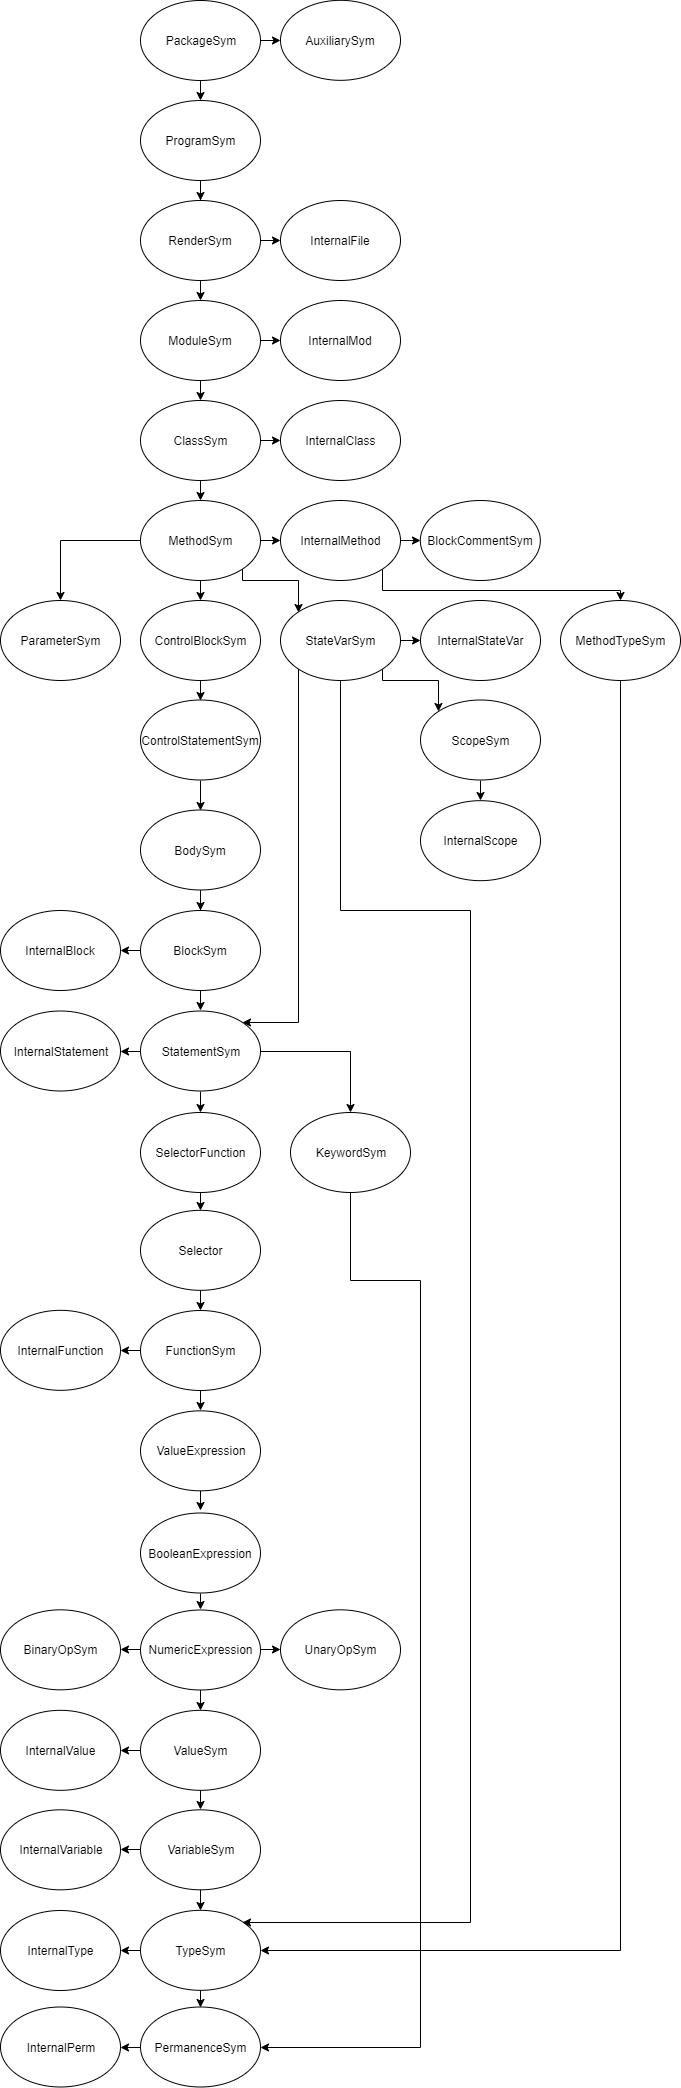
\includegraphics[scale=0.12]{GOOLClasses.png}
\end{frame}

\begin{frame}
\begin{columns}
\begin{column}{0.5\textwidth}
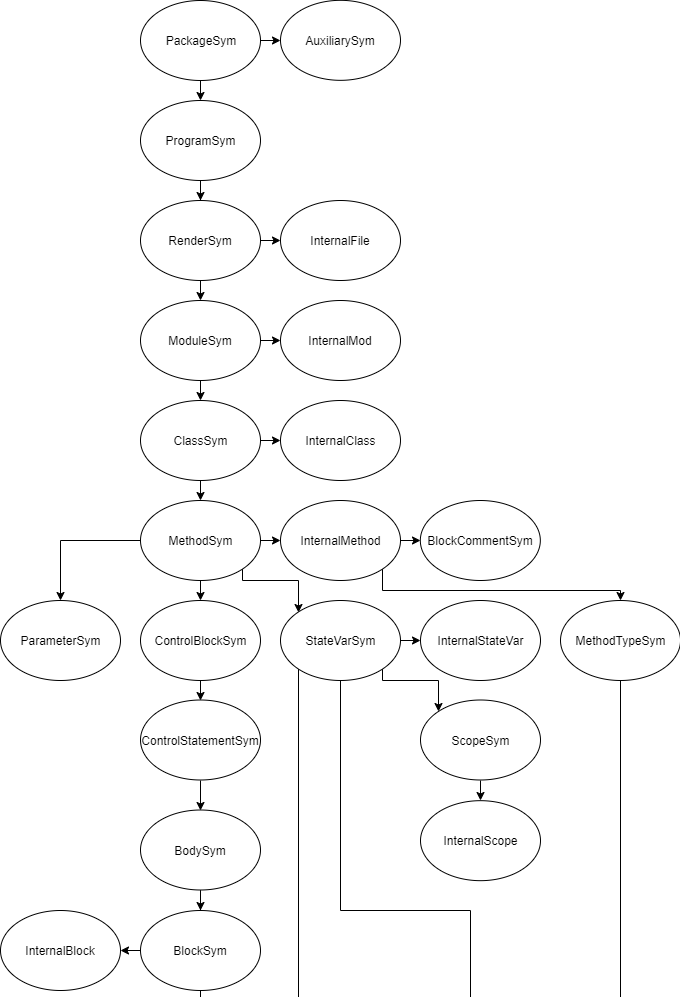
\includegraphics[scale=0.28]{GOOLClasses_top.png}
\end{column}
\begin{column}{0.5\textwidth}
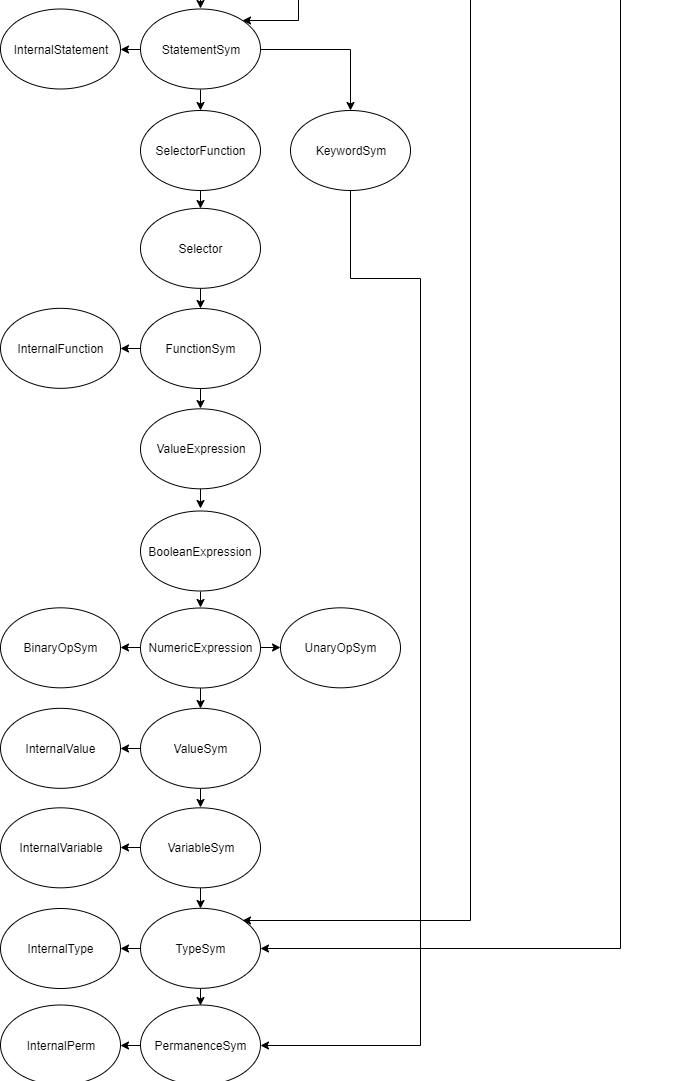
\includegraphics[scale=0.28]{GOOLClasses_bottom.png}
\end{column}
\end{columns}
\end{frame}

%%%%%%%%%%%%%%%%%%%%%%%%%%%%%%%%%%%%%%

\begin{frame}

\frametitle{Statistics}

\begin{itemize}
  \item 43 classes, 328 methods
  \item 300 functions that abstract over commonalities
  \item 40\% more common methods between Java and \Csharp~than Java and Python
\end{itemize}

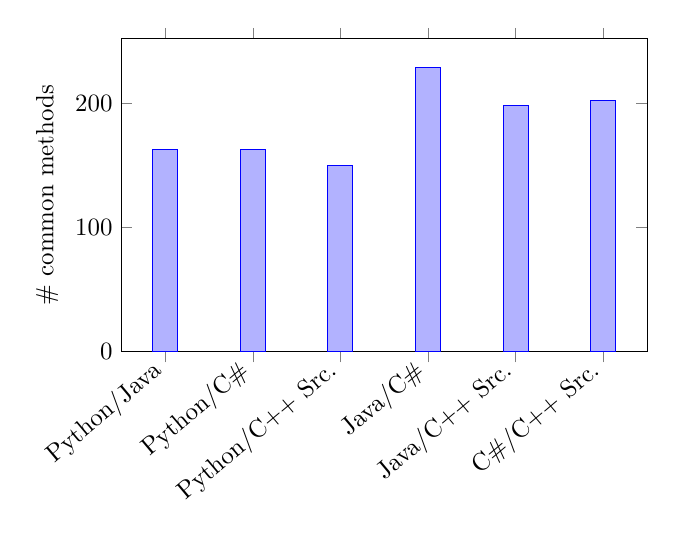
\begin{tikzpicture}[scale=0.9]
\begin{axis}[
ybar,
ymin=0,
ylabel={\# common methods},
symbolic x coords={Python/Java,Python/C\#,Python/C++ Src.,Java/C\#,Java/C++ 
	Src.,C\#/C++ Src.},
xtick=data,
x tick label style={rotate=40,anchor=east},
]
\addplot coordinates {(Python/Java,163) (Python/C\#,163) (Python/C++ Src.,150) 
	(Java/C\#,229) 
	(Java/C++ Src., 198) (C\#/C++ Src., 202)};
\end{axis}
\end{tikzpicture}

\end{frame}

%%%%%%%%%%%%%%%%%%%%%%%%%%%%%%%%%%%%%%

\section[Patterns]{Patterns}

%%%%%%%%%%%%%%%%%%%%%%%%%%%%%%%%%%%%%%

\begin{frame}

\frametitle{Things we need/want to say}

\begin{itemize}
  \item Command line arguments
  \item Lists
  \item I/O
  \item Procedures with Input/Output/Both parameters
  \item Getters and setters
  \item Design patterns
\end{itemize}

\end{frame}

%%%%%%%%%%%%%%%%%%%%%%%%%%%%%%%%%%%%%%

\begin{frame}[fragile]

\frametitle{Example: List Slicing}

GOOL: {\footnotesize \emph{hideous, we know}}
% new list, old list, start value, end value, step size
\begin{lstlisting}
listSlice sliced (valueOf old) (Just $ litInt 1)
  (Just $ litInt 3) Nothing
\end{lstlisting}
\vspace{\baselineskip}

\begin{overprint}
\onslide<1>
Python:
\begin{lstlisting}[language=Python]
sliced = old[1:3:]
\end{lstlisting}

\onslide<2>
Java:
\begin{lstlisting}[language=java]
ArrayList<Double> temp = new ArrayList<Double>(0);
for (int i_temp = 1; i_temp < 3; i_temp++) {
    temp.add(old.get(i_temp));
}
sliced = temp;
\end{lstlisting}

\onslide<3>
\Csharp:
\lstset{language=[Sharp]C}
\begin{lstlisting}
List<double> temp = new List<double>(0);
for (int i_temp = 1; i_temp < 3; i_temp++) {
    temp.Add(old[i_temp]);
}
sliced = temp;
\end{lstlisting}

\onslide<4>
\Cplusplus:
\lstset{language=C++}
\begin{lstlisting}
vector<double> temp(0);
for (int i_temp = 1; i_temp < 3; i_temp++) {
    temp.push_back(old.at(i_temp));
}
sliced = temp;
\end{lstlisting}
\end{overprint}

\end{frame}

\lstset{language=haskell}
%%%%%%%%%%%%%%%%%%%%%%%%%%%%%%%%%%%%%%

\begin{frame}[fragile]

\frametitle{Example: Setters}

GOOL:
\begin{lstlisting}
setMethod "FooClass" foo
\end{lstlisting}
\vspace{\baselineskip}

\begin{onlyenv}<1>
Python:
\begin{lstlisting}[language=Python]
def setFoo(self, foo):
    self.foo = foo
\end{lstlisting}
\end{onlyenv}

\begin{onlyenv}<2>
Java:
\begin{lstlisting}[language=java]
public void setFoo(int foo) throws Exception {
    this.foo = foo;
}
\end{lstlisting}
\end{onlyenv}

\begin{onlyenv}<3>
\Csharp:
\lstset{language=[Sharp]C}
\begin{lstlisting}
public void setFoo(int foo) {
    this.foo = foo;
}
\end{lstlisting}
\lstset{language=haskell}
\end{onlyenv}

\begin{onlyenv}<4>
\Cplusplus:
\begin{lstlisting}[language=C++]
void FooClass::setFoo(int foo) {
    this->foo = foo;
}
\end{lstlisting}
\end{onlyenv}

\end{frame}

%%%%%%%%%%%%%%%%%%%%%%%%%%%%%%%%%%%%%%

\section[Conclusions]{Conclusions}

%%%%%%%%%%%%%%%%%%%%%%%%%%%%%%%%%%%%%%

\begin{frame}

\frametitle{Future}

\begin{itemize}
  \item More types
  \item Smarter generation using State monad - ex. import statements
  \item Interface with external libraries
  \item User-decisions - ex. which type to use for lists?
  \item More patterns
\end{itemize}

\bmac{Split into a slide for each? Or pick a couple important ones and just do 
a slide for each of those?}

\end{frame}

%%%%%%%%%%%%%%%%%%%%%%%%%%%%%%%%%%%%%%

\begin{frame}

\frametitle{Language of Design}

Drasil project
\begin{itemize}
\item Generate scientific software
\item Design language allows users to influence design
\item GOOL is the backend
\end{itemize}

\end{frame}

%%%%%%%%%%%%%%%%%%%%%%%%%%%%%%%%%%%%%%

\begin{frame}

\frametitle{Complete Example}

Projectile program\\~\

\href{https://github.com/JacquesCarette/Drasil/tree/projectileDemos/Presentations/PEPM2020/projectile1}{Design
 1}
\begin{itemize}
	\item Documented
	\item Bundled inputs
\end{itemize}

\href{https://github.com/JacquesCarette/Drasil/tree/projectileDemos/Presentations/PEPM2020/projectile2}{Design
 2}
\begin{itemize}
	\item Logging
	\item More modular
\end{itemize}

\end{frame}

%%%%%%%%%%%%%%%%%%%%%%%%%%%%%%%%%%%%%%

\begin{frame}

\frametitle{Conclusion}

We currently use GOOL to generate some examples of scientific software (glass 
breakage, projectile simulation)\\~\

Together new:
\begin{itemize}
  \item Idiomatic code generation
  \item Human-readable, documented code generation
  \item Coding patterns are language idioms\\~\
\end{itemize}

With respect to ``The Goal'' --- It is possible\\~\

\end{frame}

\end{document}
